\documentclass{scrartcl}
\usepackage[ngerman]{babel} 
\usepackage[T1]{fontenc} 
\usepackage[utf8]{inputenc} 
\usepackage{amsmath} 
\usepackage{graphicx}
\usepackage{amssymb}
\usepackage{hyperref}
\usepackage[normalem]{ulem}
\usepackage{empheq}
\usepackage{xcolor}
\usepackage{dsfont}

%layout optionen
\definecolor{lblue}{HTML}{88E6FF}

%Coms
\renewcommand{\labelitemi}{$\rightarrow$}
\newcommand{\holine}{\noindent\makebox[\linewidth]{\rule{\paperwidth}{0.4pt}}} 
\newcommand{\M}{\mathbb} 
\newcommand{\T}{\text} 
\newcommand{\D}{\cdot} 
\newcommand{\pdiff}[2]{\frac{\partial #1}{\partial #2}}
\newcommand{\diff}[2]{\frac{\text{d} #1}{\text{d} #2}}
\newcommand{\mybox[1]}{\colorbox{red}{\hspace{1em}#1\hspace{1em}}}
\newcommand{\emalign}[1]{\begin{empheq}[box=\colorbox{lblue}]{flalign}
#1
\end{empheq}}
\newcommand{\half}{\frac{1}{2}}
\newcommand{\const}{\text{const.}}
\newcommand{\ges}{\text{ges}}
\newcommand{\sumni}{\sum_{i=1}^{N}}
\newcommand{\sumij}{\sum_{i,j=1; j\neq i}^{N}}
\newcommand{\skizze}[1]{
	\begin{figure}[h]
		\begin{center}
			
\includegraphics[width=0.4\textwidth]{skizze.jpg}
		\end{center}
		\caption{#1}
	\end{figure}
}
\newcommand{\desc}[1]{\item[#1]~\par}


\begin{document}

\title{Theoretische Mechanik}
\author{Till Hanke}
\date{Letzte Aktualisierung: \today}

\maketitle
\tableofcontents

\section{Raum und Zeit}

\subsection{Raum}
Die Mechanik spielt sich im dreidimensionalen Raum ab. Affiner Raum $\M{E}^3$: Menge aller Punkte im Raum.
Ein Punkt $P\in\M{E}^3$ wird durch Angabe eines Ortsvektors $\vec{r}\in\M{R}^3$ (3D-Vektorraum) relativ zu einem Ursprung $O\in\M{E}^3$ Festgelegt: $\vec{OP}=\vec{P}$.
\begin{figure}[h]
\begin{center}
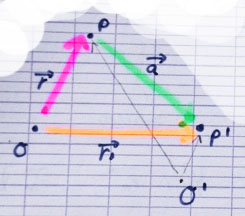
\includegraphics[width=0.4\textwidth]{Skizzen/Anhang13.jpg}
\end{center}
\caption{}
\end{figure}

Ein Skalarprodukt $\vec{r}\cdot\vec{r'}\in\M{R}^3$ liefert Längen $\Rightarrow|\vec{r}|=\sqrt{\vec{r}\D\vec{r}}$\\
und Abstände $d(P,P')=|\vec{a}|=|\vec{r}-\vec{r'}|=\sqrt{(\vec{r}-\vec{r'})\D\vec{r}-\vec{r'}}$

'Euklidischer' Raum $\M{E}^3$: affine, 3D Räume mit $d(P,P')$
\begin{description}
\item[Bemerkung]~\par
\begin{itemize}
\item Die Wahl von O ist beliebig; eine andere Wahl O' mag
  zweckmäßiger sein, „ändert nichts an der Physik“.  Insbesondere
  gilt: $d_{O}(P,P')=d_{O'}(P,P')$
\item Übergang $O\rightarrow O'$: Wechsel des Bezugssystems
\end{itemize}
\end{description}

\subsection{Koordinatensysteme}
Für $P\in\M{E}^3$ muss angegeben werden: Ursprung $O$ und Koordinaten $(x,y,z)$ bzgl. einer kartesischen OB $(e_1,e_2,e_3)$ -- Da OB: $e_i\D e_j=\delta_{ij}$ sowie $|e_i|=1$\\

Für den Punkt $P$ folgt dann:
\begin{align*}
\vec{OP}=\vec{r}=x\vec{e_1}+y\vec{e_2}+z\vec{e_3}=\sum_i^3 x_i\vec{e_i}
\end{align*}
Dem Punkt $P$ ordnen wir den Spaltenvektor $\vec{x}=\begin{pmatrix}
x \\ 
y \\ 
z
\end{pmatrix} $, bezogen auf $(O,\vec{e_1},\vec{e_2},\vec{e_3})$, zu.
\begin{description}
\item[Bemerkungen]~\par
\begin{enumerate}
% TODO Was ist mit diesem Absatz gemeint?
\item Die Wahl von $(\vec{e_1},\vec{e_2},\vec{e_3})$ ist beliebig.\\
  Es gilt: $(\vec{e_1},\vec{e_2},\vec{e_3})\rightarrow(\vec{e_1'},\vec{e_2'},\vec{e_3'})$\\
  $\vec{e_k}=\sum_i R_{ki} \vec{e_i}$ mit einer orthogonalen
  Transformation $R\in O(3)$ Drehungsmatrix $R^{-1}=R^T; (\det R=1)$
\item Transformation der Koordinaten bezogen auf $(O,\vec{e_1},\vec{e_2},\vec{e_3})$
\end{enumerate}
\end{description}

\begin{description}
\item[Aktive Transformation]~\par
\begin{itemize}
% TODO Was bedeutet „Rel. GL(")“?
\item die Rel. GL(") definiert bzgl. eines festen Koordinatensystems
  $(O,e,e,e)$ eine aktive Drehung $R$ des Vektors
  $\vec{r}=\sum_k x_k\vec{e}_k \rightarrow \vec{r'}=\sum_k
  x'_k\vec{e_k}=R\vec{r}$
\end{itemize}
\begin{figure}[h]
\begin{center}
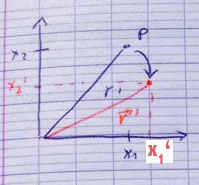
\includegraphics[width=0.4\textwidth]{Skizzen/Anhang11.jpg}
\end{center}
\caption{}
\end{figure}
\textbf{Achtung}:

Für die Basisvektoren aus Bemerkung 2 gilt: $\vec{e_k'}=(R^{-1})\vec{e_k}$ (siehe Vorübung).
\item[Transformation] Die Trafo GL(") definiert allgemein das Transformationsverhalten eines Vektors (Tensor 1.Stufe)

Beispiele:
$\vec{v}=\diff{\vec{r}}{t} \rightarrow v_k'=\sum_iR_{ki}v_i$; Geschwindigkeit, Beschleunigung, etc.\\
Bedeutung: Physikalische Grundgleichungen müssen das Trafo Verhalten respektieren

Bsp: $m\ddot{\vec{r}}=\vec{F}$. In $(O,e,e,e)$: $m\ddot{x_i}=F_i \Rightarrow$ in $(O,e',e',e')$: $m\ddot{x_i'}=F_i'$
\item[Krummliniges Koordinatensystem] in dem $x_i=x_i(q_1,q_2,q_3),i \in \left\{ 1,2,3 \right\}$ mag sinnvoll sein.

Beispiele: Zylinder- $(r, \varphi, z)$ oder Kugelkoordinaten $(r, \Theta, \varphi)$\\
\textbf{Achtung}: $\vec{e_i}\rightarrow\vec{e_i}(q_1,q_2,q_3)$
\end{description}
%\newpage

\subsection{Zeit}
\subsubsection{Ereignis}
$E$ ist ein Punkt der Raum-Zeit mit Koordinaten $(t,x,y,z)$ bezogen auf $(O,e,e,e)$
\begin{figure}[h]
\begin{center}
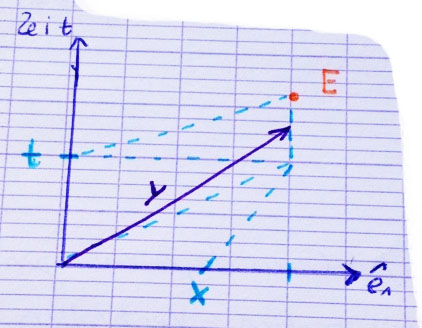
\includegraphics[width=0.4\textwidth]{Skizzen/Anhang10.jpg}
\end{center}
\caption{}
\end{figure}
\paragraph*{Ort}
räumliche Koordinaten $(x,y,z)$ werden abgelesen durch Maßstäbe.
\paragraph*{Zeit}
zeitliche Koordinate $t$ (Koordinatenzeit): abgelesen von einer Uhr\\
\begin{itemize}
\item Festlegung der Zeit $t$ eines Ereignisses durch gleichzeitiges betrachten von E und der Uhr
\item Nur lokal möglich
\item Wir denken uns den gesamten Raum ausgestattet mit Uhren, die alle synchronisiert sind.\\
\end{itemize}
Die Koordinatenzeit $t$ des Ereignisses E mit $(t,x,y,z)$ wird von der Uhr mit räumlichen Koordinaten $(x,y,z)$ abgelesen!

\subparagraph*{Bemerkung} 
\begin{enumerate}
\item Die absolute Uhrzeit $t$ ist beliebig, eine andere Wahl $t'=t+t_0$ mag zweckmäßiger sein. „Ändert nichts an der Physik“
\item Uhrensynchronisation kann durch Lichtpulse realisiert werden („Einstein-Synchronisation“), etwa vom Mittelpunkt zwischen zwei Uhren.\\
es zeigt sich: Äquivalent dazu (sehr langsamer) Uhrentransport
\item Vorsicht ist geboten beim Vergleich von Uhren in relativ zueinander bewegten Bezugssystemen
\end{enumerate}

\subsection{Kinematik}
Hier betrachtet: Kinematik der klassischen Mechanik\\
Kinematik ist die „Beschreibung der Bewegung“ -- zunächst ohne auf Ursachen einzugehen.
\begin{description}
\item[Bahnkurve] $\vec{r}(t)$
\item[Ortsvektor] % TODO Was gehört hier hin?
\item[Geschwindigkeit] o$\vec{v}(t)=diff{}{t}\vec{r}(t)$\\
$\vec{v}(t)=\vec{v}(t)\D \vec{T}(t)$ mit $|\vec{T}|=1; v(t)=|\vec{v}(t)|$
\item[Beschleunigung] $\vec{a}(t)=diff{}{t}\vec{v}(t)=\dot{t}\vec{T}+v(t)\dot{\vec{T}}(t)$

\begin{figure}[h]
\begin{center}
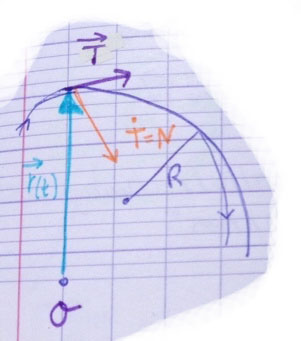
\includegraphics[width=0.4\textwidth]{Skizzen/Anhang9.jpg}
\end{center}
\caption{}
\end{figure}
\end{description}
$\vec{N}=\frac{\dot{\vec{T}}(t)}{|\dot{\vec{T}}(t)|}$ steht senkrecht auf $\vec{T}$ und $|\vec{N}|=1$ („Normalenvektor)\\
$(T,N)$ definieren „Schmiegeebene“, in der lokal die Bahnkurve durch einen Kreis mit Krümmungsradius $R=\frac{v}{|\dot{\vec{T}}|}$ beschrieben werden kann (siehe Übung).\\
Es folgt $\vec{a}=\dot{v}\vec{T}+\frac{v^2}{R}\vec{N}$ als Summe von zwei orthogonalen Beiträgen -- wobei
\begin{itemize}
\item Der erste: Eine \emph{Tangentialbeschleunigung} und
\item Der zweite: Eine \emph{Normal- oder Zentripetalbeschleunigung}
\end{itemize}
ist.

%\newpage

\begin{description}
\item[Beispiel]~\par
\begin{enumerate}
\item Geradlinig-gleichförmige Bewegung 
\begin{align*}
  \vec{r}(t)=\vec{r_0}+\vec{v_0}t \quad
  \Rightarrow\vec{a}=0 \qquad
  (\dot{v}=0, R=\infty)
\end{align*}
\begin{figure}[h]
\begin{center}
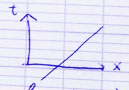
\includegraphics[width=0.4\textwidth]{Skizzen/Anhang8Kopie.jpg}
\end{center}
\caption{}
\end{figure}
\item Geradlinige Bewegung (allgemein)
\begin{align*}
\vec{r}(t)=\vec{r_0}+l(t)\vec{T_0},\qquad
\vec{v}=\dot{l}\: \vec{T_0} \Rightarrow v=\dot{l}, \quad
\vec{T}=\vec{T_0} \qquad
(\dot{v}=\ddot{l}; R=\infty)
\end{align*}
\begin{figure}[h]
\begin{center}
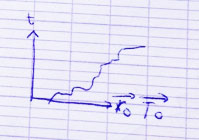
\includegraphics[width=0.4\textwidth]{Skizzen/Anhang8.jpg}
\end{center}
\caption{}
\end{figure}
\item Gleichförmige Kreisbewegung
\begin{align*}
v&=\frac{2\pi R}{\tau} = const.\\
\dot{v}&=0\\
\vec{a}&=\frac{v^2}{R}\D \vec{N}=4\pi^2\frac{R}{\tau^2}\vec{N}
\end{align*}
Mit $\tau$ Umlaufzeit\\

\begin{figure}[h]
\begin{center}
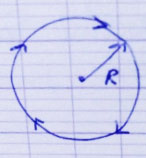
\includegraphics[width=0.4\textwidth]{Skizzen/Anhang7.jpg}
\end{center}
\caption{}
\end{figure}
Anwendung auf Kepler-Bahnen für Planeten $\tau^2\sim R^3$ (3.Keplergesetz):\\
$\Rightarrow\vec{a}\sim \frac{1}{R^2}\vec{N}$ ($\vec{F}=m\vec{a}) \Rightarrow$ Planetenbewegung $\vec{F}\sim \frac{1}{R^2}\vec{N}$

\end{enumerate}
\end{description}

\subsection{Bewegte Bezugssysteme und Inertialsysteme}
\begin{itemize}
\item Bezeichne RS das Ruhesystem
\item Wie wählen wir $(O,e_1,e_2,e_3)$ \emph{geeignet}? $\Rightarrow$
  Nahe liegend: \emph{Laborsystem} (Labortisch ruht im LS)
\item \emph{Beispiel} elastischer Stoß im LS ($m$ ruht)
\end{itemize}
\begin{figure}[h]
\begin{center}
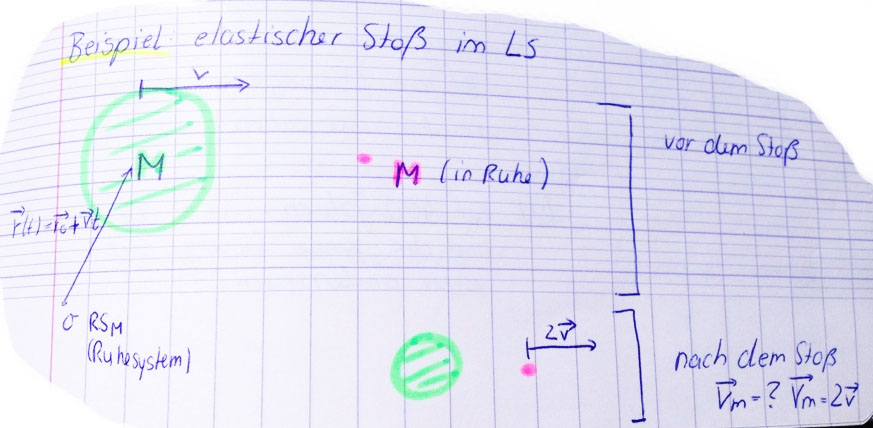
\includegraphics[width=0.4\textwidth]{Skizzen/Anhang6.jpg}
\end{center}
\caption{}
\end{figure}
%\newpage

Wechsle ins Ruhesystem der Masse $M$\\
Die Betrachtung wird eindeutig und trivial bei $M\gg m$\\
%TODO reformat
Übergang von System Labortisch (O,e,e,e, Uhren) in RS der großen Masse M (O',e',e',e', Uhren') gilt:
\begin{align*}
\vec{r'}=\vec{r}-\vec{v}t\\
t'=t
\end{align*}
\begin{figure}[h]
\begin{center}
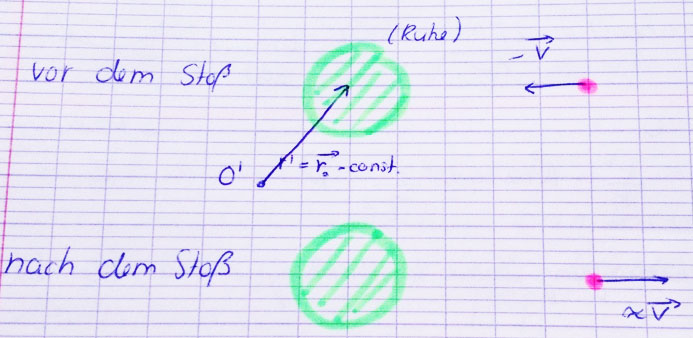
\includegraphics[width=0.4\textwidth]{Skizzen/Anhang5.jpg}
\end{center}
\caption{}
\end{figure}

Die \textbf{Galilei-Transformation} beschreibt Transformationsgesetz von BS zu BS', das sich mit Geschwindigkeit $v$ relativ zu BS bewegt. Zur Beschreibung sind $BS=RS_m$ und $BS'=RS_M$ völlig gleichwertig (hier $BS'$ transparenter).\\
\subparagraph*{Bemerkungen}
\begin{enumerate}
\item Zustand \textbf{„in Ruhe“} hat keine Absolute Bedeutung sondern
  hängt von der Wahl des Bezugssystems ab. (Bewegung ist
  \emph{relativ} zu sehen)
\item Frage vor 400 Jahren: Ruht die Erde und die Sonne bewegt sich?\\
  Galilei: Frage ist bedeutungslos, nicht entscheidbar\\
  $\Rightarrow$ Galilei-Transformationen
\item Relativität kommt zum Ausdruck im 1. Newtonschen Gesetz:(„Trägheitssatz“)\\
Ein Körper verharrt im Zustand der Ruhe oder der geradlinig-gleichförmigen Bewegung sofern er nicht durch Kräfte zur Änderung gezwungen wird.
\end{enumerate}

\subsubsection{Inertialsysteme}
(IS) sind BS, die durch die Gültigkeit des 1. Newtonschen Gesetzes ausgezeichnet sind. Ausgehend von einem IS findet man weitere IS' durch geradlinig-gleichförmige Bewegung des IS' relativ zu IS. (häufig IS='ruhend bzgl. des Fixsternhimmels'; in der Praxis LS$\approx$IS (gute Näherung)).\\
in einem relativ zu IS \underline{beschleunigten} BS treten \underline{Scheinkräfte} auf, die nicht auf fundamentalen Wechselwirkungen (Coulombkraft, etc) beruhen.\\
$\Rightarrow$ physikalische Grundgesetze werden bzgl. eines IS
formuliert, dabei sind \underline{alle} IS völlig gleichwertig;
IS$\rightarrow$IS' durch:
\begin{enumerate}
\item „Boost“ mit Richtung $\vec{v}$ $t'=r(t-\frac{\vec{v}\vec{r}}{c^2})$
\item Gleichförmig-geradlinige Bewegung: $\vec{r'}=\vec{r}-\vec{v}t$ (3 Parameter)\\
(Galilei-Relativität)
\item Räumliche Verschiebung: $\vec{r'}=\vec{r}+\vec{r_0}$ (3 Parameter)\\
(Homogenität des Raumes)
\item Räumliche Drehung: $\vec{r'}=R\vec{r}$ (3 Parameter)\\
(Isotropie des Raumes)
\item Zeitgleiche Verschiebung: $t'=t+t_0$ (1 Parameter)\\
(Homogenität der Zeit)
\end{enumerate}
Die Kombination all dieser Transformationen definieren die
\emph{'Galilei-Gruppe'} der klassischen Raum-Zeit mit 10 freien
Parametern.
\subsection{Galilei- und Lorenztransformationen}
Die Naturgesetze müssen von einer Art sein, die (Form-)invariant sind unter Transformation zwischen IS\\
Bsp.: IS$\rightarrow$IS', dann gilt für Newton:\\
\begin{equation*}
  m\frac{d^2 \vec{r}}{dt^{2}}=\vec{F} \Leftrightarrow m\frac{d^{2}\vec{r'}}{dt'^{2}}=\vec{F'}
\end{equation*}
$\rightarrow$ \emph{Relativitätsprinzip!} Insbesondere gilt:\\
geradlinig-gleichförmige Bewegung in IS mit Koordinaten(t,x,y,z) ist
auch eine geradlinig-gleichförmige Bewegung in einem anderen IS' mit
(t',x',y',z').

\begin{description}
\item[Bsp: Galilei-Transformaiton]: mit $\vec{v}$ rel. zu IS bew. IS' gilt $\vec{r'}=\vec{r}-\vec{v}t$, $t'=t+t_0$\\
  in IS: $\vec{r}(t)=\vec{r_0}+\vec{u}t$\\
  $\Rightarrow IS': \vec{r'}(t')=\vec{r_0}+(\vec{u}-\vec{v})t'$\\
\item[Umkehrung?] folgt aus der Forderung (s.o.) dass $t,\vec{r}\rightarrow t',\vec{r'}$ eine Galilei-Trafo?\\
  Frage: 'wie sieht allgemein eine Trafo
  $(t,x,y,z)\rightarrow(t',x',y',z')$ aus, die die Forderung (s.o.)
  erfüllt für IS$\rightarrow$IS', das sich mit $\vec{v}$ (vorgegeben)
  relativ zu IS bewegt?
\begin{figure}[h]
\begin{center}
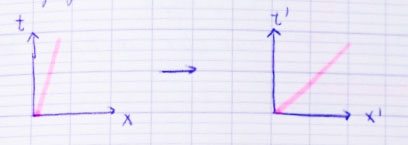
\includegraphics[width=0.4\textwidth]{Skizzen/Anhang4.jpg}
\end{center}
\caption{}
\end{figure}
\begin{itemize}
\item lineare Trafo der Raum-Zeit! $\begin{pmatrix}
t'\\
x'\\
y'\\
z'
\end{pmatrix}
=\begin{pmatrix}
. & . & . & . \\
.\\
. & 4 & \times & 4\\
.
\end{pmatrix}
\begin{pmatrix}
t\\
x\\
y\\
z
\end{pmatrix}
$
\item bzgl. räumlicher Anteile $\vec{r}$ Vektorcharakter muss erhalten bleiben: $\vec{r'}\sim\vec{r},\vec{v}$
\item Ansatz:
  \begin{align*}
t'=a	(v)			t+b(v) 			(\vec{v}\D \vec{r})\\
\vec{r'}=c(v)		\vec{r}+\frac{d(v)}{v^2}	(\vec{v}\D\vec{r})\vec{v}+e(v)		\vec{v}t
\end{align*}
mit beliebigen Funktionen $a(v),\cdots,e(v)$, die bestimmen weitere
Forderungen:
\end{itemize}
\begin{enumerate}
\item für $\vec{r}=\vec{v}t \Rightarrow \vec{r'}=0 \Rightarrow c+d+e=0$
\item Relativität (I) Vertausche Rolle IS$\leftrightarrow$IS' ($\vec{v}\rightarrow-\vec{v}$)\\
\begin{align*}
\Rightarrow t=a(v)t'-b(v)(\vec{v}\vec{r'})\\
\vec{r}=c(v)\vec{r'}+\frac{d(v)}{v^2}(\vec{v}\D\vec{r'})\vec{v}+e(v)\vec{v}t'
\end{align*}
ersetze $t'$ und $\vec{r'}$ auf der rechten Seite durch Ansatz\\
\begin{align*}\Rightarrow t=a(v)(a(v)t+b(v)(\vec{v}\vec{r})-...\\
\vec{r}=c(v)(c(v)\vec{r}+...)+...\vec{v}...\\
\Rightarrow c^2=1; a=c+d; a^2=1+ebv^2; e=-a\\
\Rightarrow c=1; e=-a; d=a-1; b=\frac{1-a^2}{av^2}
\end{align*}
Wähle Koordinatensystem so, dass x in Richtung $\vec{v}$ zeigt.
$\Rightarrow \vec{v}=\begin{pmatrix}
v\\
0\\
0
\end{pmatrix}$
\begin{align*}
t'=a(v)t+\frac{1-a^2(v)}{a(v)v}x\\
x'=a(v)(x-vt); y'=y; z'=z
\end{align*}
\item Relativitätsprinzip:\\
IS$\rightarrow^v$ IS'$\rightarrow^u$ IS''\\
\begin{align*}
t'' &=a(u)t'+\frac{1-a^2(u)}{a(u)u}x'=a(u)(a(v)t+\frac{1-a^2(v)}{a(v)v}x)+\frac{1-a^2(u)}{a(u)u}(a(v)(x-vt))\\
x'' &=a(u)(x'-ut')=a(u)(a(v)-u\frac{1-a^2(v)}{a(v)v})x+...t
\end{align*}
außerdem muss gelten IS$\rightarrow^w$ IS''\\
woraus folgt, dass
\begin{align*}
t''=a(w)t+(w)x\\
x''=a(w)(x-wt)
\end{align*}
woraus dann folgt:
\begin{align*}
[a(u)a(v)-\frac{va(v)}{ua(u)}			&(1-a^2(u)]t+...x \\
a(u)a(v)-\frac{va(v)}{ua(u)}(1-a^2(u) 	&=a(w)\\
\Rightarrow\frac{a^2(u)-1}{u^2a^2(u)} 	&=\frac{a^2(v)-1}{v^2a^2(v)}\\
\Rightarrow \frac{a^2(v)-1}{v^2a^2(v)} 	&=const.=K \\
\Rightarrow a(v) 						&=\frac{1}{\sqrt{1-Kv^2}}\\
 k=0\Rightarrow a=1 						&\Rightarrow \text{ist Galilei Trafo}\\
 k\neq 0? [k]=\frac{1}{\text{Geschwindigkeit}^2} &=\frac{1}{c^2}=const.
\end{align*}

\begin{align*}
 \Rightarrow &t'=a(v)(t-\frac{vx}{c^2})\\
 &x'=a(v)(x-vt)
\end{align*}
Die Lorentz-Transformation mit $a(v)\rightarrow \gamma(v)=\frac{1}{\sqrt{1-\frac{v^2}{c^2}}}$\\
Bedeutung von $c$?\\
Man betrachte die 'Addition' von Geschwindigkeiten: $w=u+v$?
\begin{align*}
a(w)		&=a(v)a(u)(1+kuv)\\
1-kw^2	&=\frac{(1-kv^2)(1-ku^2)+(1+kuv)^2-(1+kuv)^2}{(1+kuv)^2}\\
		&=1-k\frac{(u+v)^2}{(1+kuv)^2}\\
\Rightarrow w	&=\frac{u+v}{1+kuv}\Leftrightarrow(\frac{w}{c})^2\\
		&=\frac{(\frac{u}{c}+\frac{v}{c})^2}{(1+\frac{uv}{c^2})^2}\\
		&=1-\frac{(1-\frac{u}{c}^2)(1-\frac{v}{c}^2)}{(1+\frac{u}{c}\frac{v}{c})^2}
\end{align*}
\underline{Folgerungen}:
\begin{enumerate}
\item für $u=c\Rightarrow w=c$
\item für $v=c\Rightarrow w=c$
\item für $u<c; v<c \Rightarrow w<c$
\item für $u\ll c; v\ll v \Rightarrow w\approx u+v$
\end{enumerate}
$c$ ist Lichtgeschwindigkeit
\end{enumerate}
\subparagraph*{Raum-Zeit-Diagramme}
\begin{figure}[h]
\begin{center}
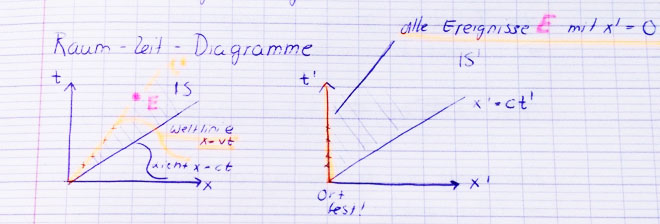
\includegraphics[width=0.4\textwidth]{Skizzen/Anhang3Kopie.jpg}
\end{center}
\caption{}
\end{figure}
\end{description}
%%% Local Variables:
%%% mode: latex
%%% TeX-master: "Script"
%%% End:

\section{Newtonsche Mechanik}
\begin{itemize}
\item basiert auf Galilei-Raum-Zeit (gültig für $v\ll c$) $m\ddot{\vec{r}}=\vec{F}(\vec{r})$ 'Fernwirkung' der Kraft $\leftrightarrow$ Widerspruch zur Vorstellung einer endlichen Ausbreitungsgeschwindigkeit von Wirkungen.
\item relativistische Mechanik folgt in Kap.7 
\end{itemize}
\subsection{Newtonsche Bewegungs-Gleichung}
zunächst phänomenologisch; Erfahrung: durch angabe des Anfangsortes $\vec{r}(t_0)=\vec{r}$ und der Anfangsgeschwindigkeit $\dot{\vec{r}}(t_0)=\vec{v_0}$ die Bahnkurve $\vec{r}(t)$ festgelegt ist $\Rightarrow$ wir erwarten eine Relation $\ddot{\vec{r}}(t) \sim \vec{F}(\vec{r},\dot{\vec{r}})$, gewöhnliche Differentialgleichung 2. Ordnung zur Bestimmung der Bahnkurve $\vec{r}(t)$ (Dynamik)\\
$\rightarrow$ Newton (2. Newton-Gesetz); Impuls $\vec{p}=v\vec{v}=\dot{\vec{r}}$\\
$\frac{d}{dt}\vec{p}=\vec{F}$, bei konstanter (träger) Masse $m\ddot{\vec{r}}=\vec{F}$ wobei $\vec{F}$ die Kraft ist, die auf den Körper wirkt.\\
\begin{description}
\item[Beispiel:]
\begin{enumerate}
\item gglf. Bew. \\
$\vec{F}=0 \Leftrightarrow \ddot{\vec{r}}=0 \Rightarrow \vec{r}(t) = \vec{r_0}+\vec{v_0}(t-t_0)$
\item $\vec{F}=\vec{F_0}$ konstant (Gewichtskraft in der Nähe der Erdoberfläche) \\
$\vec{r}(t)=\vec{r_0}+\vec{v_0}(t-t_0)+0,5 \frac{\vec{F_0}(t-t_0)}{m}$ (Wurfparabel)
\item Federkraft (1Dim) \\
$m\ddot{x}=-kx, F(x)=-kx, w^2=\frac{k}{m}\Rightarrow x(t)=x_0cosw(t-t_0)+\frac{v_0}{w}sinw(t-t_0)$
\item Lorenzkraft geschwindigkeits-abhängig \\
$\vec{F}=q(\vec{E}+\frac{\dot{\vec{r}}}{c}\times\vec{B}); \vec{E}=\vec{E}(\vec{r},t); \vec{B}=\vec{B}(\vec{r},t)$
\item Reibungskräfte (phänomenologisch) \\
$\vec{F_R}=-\alpha\dot{\vec{r}}; \alpha>0$ Reibungskoeffizient.
\item Coulombkraft\\
\begin{figure}[h]
\begin{center}
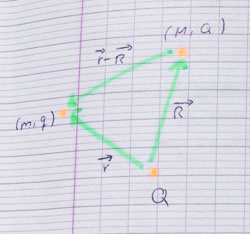
\includegraphics[width=0.4\textwidth]{Skizzen/Anhang2Kopie.jpg}
\end{center}
\caption{}
\end{figure}
$\vec{F}=cqQ\frac{\vec{r}-\vec{R}}{|r-R|^3}$\\
$qQ<0$: anziehend\\
$qQ>0$: abstoßende\\
$c$: Konstante, abhängig von der Einheit Ladung
\end{enumerate}
\end{description}
\subsection{Arbeit und Energie}
\begin{align*}
m\ddot{\vec{r}}\dot{\vec{r}}=\vec{F}\dot{\vec{r}}\\
\frac{d}{dt}(0,5m\dot{\vec{r}}^2)	\Rightarrow\int_{t_1}^{t_2}dt(\frac{d}{dt}(0,5m\dot{\vec{r}}^2))=\int_{t_1}^{t_2}dt\vec{F}\dot{\vec{r}}\\
\Rightarrow T(t_2)-T(t_1)=\int_{t_1}^{t_2}\vec{F}\frac{d\vec{r}}{dt}dt =\int_{t_1}^{t_2}\vec{F}d\vec{r}(t)
\end{align*}
Entlang der Kurve$L$ $\vec{r}(t)$ mit $r(t_1)=r_1...$
\begin{figure}[h]
\begin{center}
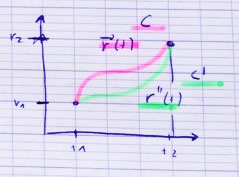
\includegraphics[width=0.4\textwidth]{Skizzen/Anhang2.jpg}
\end{center}
\caption{}
\end{figure}
Wir definieren die am Teilchen geleistete Arbeit entlang $L$ durch $W_e(r_1\rightarrow r_2)=\int_L \vec{F}d\vec{r}=\int_{t_1}^{t_2}\vec{F}\dot{\vec{r}}dt$\\
Wir nennen ein Kraftfeld $\vec{F}$ \underline{konservativ}, wenn $W_e$ nur von $r_1$ und $r_2$, aber nicht vom Weg $r(t)$ abhängt.\\
\begin{description}
\item[Theorem] $\vec{F}(\vec{r})$ konservativ $\Leftrightarrow$ es existiert ein skalares Potential $U(\vec{r})$ mit $\vec{F}(\vec{r})=-\nabla U(\vec{r})$
\begin{align*}
\Leftrightarrow \oint\vec{F}(\vec{r})d\vec{r}=0 \Leftrightarrow\nabla \times\vec{F}=0
\end{align*}
, Kraftfeld ist Wirbelfrei.
\end{description}
Für konservative Kraftfelder gilt: $\int_L F(r)dr=-U(r_2)+U(r_1)=W(r_1\rightarrow r_2)$\\
$\Rightarrow$ $T(t_2)+U(r_2)=T(t_1)+U(r_1)$\\
wir sehen für konservative Kräfte $F=-\nabla U(r)$ folgt:\\
\underline{Energieerhaltung} $E=T+U=0,5m\dot{r}+U(r(t))=const$!\\
denn $\frac{d}{dt}E=m\dot{r}\ddot{r}+\nabla U(r(t))\dot{r}(t)=\dot{r}(t)(m\ddot{r}+\nabla U)=0$ (Newton-Gleichung)
\subsubsection{Beispiele konservativer Kraftfelder}
$F=-\nabla U$\\
\begin{enumerate}
\item $F=F_0 \Rightarrow U(r)=-F_0r$
\item Federkraft $F=-kr \Rightarrow U(r)=0,5f(r\D r)=0,5kr^2$ (harmonischer Oszilator)
\item Coulombkraft, $U(r)=cqQ\frac{1}{|r-R|}$

\subsubsection{Gegenbeispiel}
\item Reibungskraft $F=-\alpha \dot{r}$ konservativ?\\
berechne Arbeit entlang einer geschlossenen Bahn:$\oint Fdr=-\alpha \oint \dot{r}dr=-\alpha \oint \dot{r}^2dt \neq 0, >0$ (außer $\dot{r}=0$)
\end{enumerate}
\subsubsection{Bemerkung}
\begin{enumerate}
\item $E=T+U; T=0,5m\dot{r}^2$ \underline{Kinetische Energie};\\
$U=U(r)$ \underline{potentielle Energie}, nur bis auf additive Konstante festgelegt (definiert das \underline{Energie-Nullniveau})
\begin{figure}[h]
\begin{center}
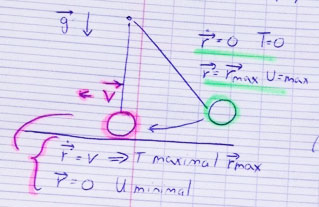
\includegraphics[width=0.4\textwidth]{Skizzen/Anhang1Kopie.jpg}
\end{center}
\caption{}
\end{figure}
\item $E=const$ wichtiger \underline{Energieerhaltungssatz}. (hängt zusammen mit Symmetrien!)
\end{enumerate}
\subsection{Systeme mehreren (N) Teilchen}
\begin{figure}[h]
\begin{center}
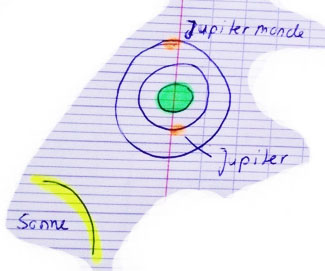
\includegraphics[width=0.4\textwidth]{Skizzen/Anhang1.jpg}
\end{center}
\caption{}
\end{figure}
Dynamik: N Punkteilchen mit Ortsvektoren $r$; $i=1$, $N$ und trägen Massen $m$; es gelten Newtons Gleichungen
\begin{align*}
m_i\ddot{r_i}=F_i (r_1,...r_N,\dot{r_1},...\dot{r_N},t)
\end{align*}
N gekoppelte Diff.-Gl. für die $r_i(t)$; Anfangsbed. $r(0); \dot{r}(0)$ müssen gegeben sein.\\
Häufig: konservative Kräfte: $F_i=-\nabla_i U(r_1,...,r_N)$ es folgt Energieerhaltung (Gesamtenergie).
\begin{align*}
E=\sum^N_{i=1} 0,5m_i\dot{r_i}^2(t)+U(r_1(t),...,r_N(t))=const\\
\nabla_i=\frac{\delta}{\delta r_i}
\end{align*}
häufig setzt sich die Kraft $F_i$ zusammen aus 'äußeren' Kräften $F_i^{(a)}$ und paarweise auftretenden 'inneren' Kräften $F_{ij}$ zwischen den $N$ Teilchen.
\begin{align*}
F_i=F_i^{(a)}(r_i) + \sum^N_{j=1; j\neq i}F_{ij}(r_i,r_j)
\end{align*}
konservative Kräfte: $F_i^{(a)}(r_i)=-\nabla_i U^{(a)}(r_1,...,r_N)$\\
und $F_{ij}=-\nabla_i\sum^N_{j=1; i\neq j}V_{ji}(|r_i-r_j|)$ für abstandsabh. Zweiwechselwirkung ($F_{ij}=-F_{ji}$)\\
es folgt Energieerhaltung in der Form:
\begin{align*}
E=\sum^N_{i=1}0,5m_i\dot{r_i}^2+U^{(a)}(r_1,...,r_N)+0,5\sum^N_{i,j=1; i\neq j}V_{ij}(|r_i-r_j|)
\end{align*}
kin Energie + äußere Pot. Energie + innere Energie
\subsection{N-Teilchenproblem}
\begin{align*}
m_i\ddot{\vec{r_i}}=\vec{F_i^{(a)}}(\vec{r_i})+\sum_{i=1, j\neq i}^{N}\vec{F_{ij}}(\vec{r_i}-\vec{r_j})
\end{align*}
\begin{figure}[h]
	\begin{center}
		
\includegraphics[width=0.4\textwidth]{skizze.jpg}
	\end{center}
	\caption{innere und äußere Kräfte}
\end{figure}
\emph{für konservative Kräfte} 
\begin{flalign}
	\vec{F_i^{(a)}}=-\vec{\nabla_i} U_i(\vec{r_i})\\
	\vec{F_{ij}}=-\vec{\nabla_i}V_{ij}(|\vec{r_i}-\vec{r_j}|)
\end{flalign}
Gesamtenergieerhaltung: $E=T+U^{(a)}+v^{WW}$\\
\paragraph{Bemerkungen:}
	\begin{enumerate}
	\item \emph{Abgeschlossene Systeme} sind solche ohne äußere Kräfte, also \\
		$\vec{F_i^{(a)}}=0, U^{(a)}=\text{const.}$
	\item \emph{Schwerpunkt} des Systems:
	\begin{flalign*}
		\vec{R_{CM}}=\frac{1}{M}\sum_{i=1}^{N}m_i\vec{r_i}, 	& M=\sum_{i}m_i\\
																& \text{Gesamtmasse}
	\end{flalign*}
	\item \emph{Trennung der Energie in Schwerpunkt und Relativteil}:
	\begin{flalign*}
		\dot{\vec{r_i}} =  \dot{\vec{R_{CM}}}+\dot{\vec{\rho_i}} & \text{ Definition von} \vec{\rho_i}\\
		T=\sum_{i=1}^{N}\frac{1}{2}m_i\dot{\vec{r_i}}2=\frac{1}{2}M\dot{\vec{R_{CM}}}^2+\dot{\vec{R_{CM}}}\cdot
		\underbrace{\sum_{i=1}^{N}m_i\dot{\vec{\rho_i}}}_{=0}+\sum_{i=1}^{N}\half m_i\dot{\vec{\rho_i}}^2\\
		\sum_{i=1}^{N}m_i\vec{r_i}=\sum_{i=1}^{N}m:i(\vec{R_{CM}}+\vec{\rho_i})=M\vec{R_{CM}}+\underbrace{\sum_{i=1}^{N}m_i\vec{\rho_i}}_{=0}\\
		T=\underbrace{T_{CM}}_{\half M\dot{\vec{R}}_{CM}^2}+T{rel}
	\end{flalign*}
	\end{enumerate}
für abgeschlossene Systeme
\begin{flalign*}
	E	&=E_{CM}\cdot E_{rel}\\
		&=T_{CM} + (T_{rel}+V^{WW})
\end{flalign*}

\subsection{Impuls und Drehimpuls}
\paragraph{Gesamtimpuls:}
\begin{flalign}
	\vec{P}_{CM}=\sum_{i=1}^{N}m_i\dot{\vec{r}}_i=M\dot{\vec{R}}_{CM}
\end{flalign}
\paragraph{Änderung:}
\begin{flalign}
	\diff{}{t}\vec{P_{CM}}=\sum_{i=1}^{N}(\vec{F_i}^{(a)}+\sum_{j=1; j\neq i}^{N}\vec{F_{ji}})\\
	=\sum_{i=1}^{N}\vec{F_i}^{(a)}+\underbrace{\sum_{i,j=1; i\neq j}^{N}\vec{F_{ji}}}_{=0\text{ (alle Kräfte und ihre Gegenkräfte)}}=\sum_{i=1}^{N}\vec{F_i}^{(a)}
\end{flalign}
\paragraph{Bemerkungen:}
\begin{enumerate}
	\item für abgeschlossene Systeme gilt Gesamtimpulserhaltung:
	\begin{flalign}
		\vec{P_{CM}}(t)=\vec{P_{CM}}(0)=\text{const.}\\
		\text{falls:}\vec{F_i}^{(a)}=0
	\end{flalign}
	\item für $\vec{R_{CM}}$ folgt für abgeschlossene Systeme: 'Schwerpunktsatz'
\\
\begin{flalign}
\vec{R_{cm}}(t)=\vec{R_{CM}}(t_0)+\frac{P{CM}(t_0)}{M}(t-t_0)
\end{flalign}
Schwerpunkt bewegt sich geradlinig-gleichförmig (für abgeschlossene Systeme)
\item Beschreibung der Dynamik ausgedehnter Pbjekte durch Punktteilchen (Schwerpunkt) ist gerechtfertigt
\item $\vec{P_{CM}}=\const$ sehr wichtig für Stoßprozesse gültig für
$\left\{
\begin{array}{cc}
	\text{elastische Stoßprozesse:}	&	E=\const	\\
	\text{inelastischer Stoß:}		&	\text{ein Teil der Enerdie geht über in Verformung}
\end{array}
\right.$
\item häufig Wahl des Schwerpunktsystems $O\rightarrow \vec{R_{CM}}$ (Ursprung) als Bezugssystem
\end{enumerate}
%
\subsubsection{Drehimpuls}
%
\begin{flalign}
\underbrace{\vec{L}=\vec{r}\times\vec{p}}_{\text{(hängt von der Wahl des Ursprungs ab)}}; 	&	\vec{p}=m\dot{\vec{r}}
\end{flalign}
%
\paragraph{zeitliche Änderung:}
%
\begin{flalign}
\diff{}{t}\vec{L}=\underbrace{(\dot{\vec{r}}\times\vec{p})}_{0}+\vec{r}\times\dot{\vec{p}}=\vec{r}\times\vec{F}=:\underbrace{\vec{M}}_{\text{Drehmoment}}\\
\ulcorner \diff{}{t}\vec{p}=\vec{F}, \diff{}{t}\vec{L}=\vec{M} \lrcorner
\end{flalign}
%
\paragraph{für N-Teilchen: Gesamtdrehimpuls}
%
\begin{flalign}
\vec{L_{\ges}}=\sum_{i=1}^{N}\vec{L_i}=\sum_{i=1}^{N}m_i(\vec{r_i}\times\vec{r_i})
\end{flalign}
%
\paragraph{Zeitliche Änderung:}
%
\begin{flalign}
	\diff{}{t}\vec{L}_{\ges}&=\sumni (\vec{r_i}\times\vec{F_i})=\sumni(\vec{r_i}\times\vec{F_i}^{(a)}+\sumij\vec{F_ij})\\
	&\Rightarrow \diff{}{t}\vec{L_{\ges}}=\underbrace{\sumni\vec{M_i}^{(a)}}_{äußeres Drehmoment}+\sumij(\vec{r_i}\times\vec{F_{ij}})\\
	&\Rightarrow \diff{}{t}\vec{L_{\ges}}=\vec{M}^{(a)}=\sumni\vec{M_i}^{(a)}
\end{flalign}
%
\paragraph{Bemerkung:}
%
\begin{enumerate}
	\item für geschlossene Systeme ($\vec{M_i}^{(a)}=0$) gilt \emph{Gesamtdrehimpulserhaltungssatz}:
		\begin{flalign}
			L_{ges}=\sumni \vec{L_i}=\const
		\end{flalign}
	\item Zerlegung in Schwerpunkt und Relativteil: $\vec{r_i}=\vec{R_{CM}}+\vec{\varrho_i}$
	\begin{flalign}
		\vec{L}=\sumni (\vec{r_i}\times\vec{p_i})=\underbrace{\vec{R_{CM}}\times\vec{P_{CM}}}_{\vec{L}_{CM}}+\underbrace{\sumni(\vec{\varrho_i}\times\vec{p_i})}_{\vec{L}_{rel}}
	\end{flalign}
	\item diese Erhaltungssätze für abgeschlossene N-Teilchensysteme gelten:\\
	\begin{flalign*}
		E & & \text{Energie} & & 1\times\\
		\vec{P_{CM}} & & \text{Gesamtimpuls} & & 3\times\\
		\vec{L_{\ges}} & & \text{Gesamtdrehimpuls} & & 3\times
	\end{flalign*}
	\emalign{
		\vec{R_{CM}}(0)=\vec{R_{CM}}(t)-\frac{\vec{P}t}{M} & & \text{Schwerpunktsatz}
		}
	$\Rightarrow$ 10 Erhaltungsgrößen für dynamik eines abgeschlossenen Systems\\
	$\leftrightarrow$ verknüpft mit der Homogenität der Zeit ($t\rightarrow t+t_0$), Homogenität des Raumes ($\vec{r}\rightarrow\vec{r}+\vec{r_0}$), Isotopie des Raumes ($\vec{r}\rightarrow R\vec{r}$)\\
	Galilei-Transformation:
	\begin{flalign*}
		r'&\rightarrow\vec{r}-\vec{v}t\\
		t&\rightarrow t
	\end{flalign*}
	\item für abgeschlossene Systeme gelten die Newtonschen-Gleichungen
	\begin{flalign*}
		& m_i\ddot{\vec{r_i}}=\sumij \vec{F_{ij}}(|r_i-r_j|) & & \text{in IS beim Übergang in IS'} &
	\end{flalign*}
	\begin{flalign*}
		\rightarrow |\vec{r_i}-\vec{r_j}|=|\vec{r_i}'-\vec{r_j}'| & & \text{mit} & & \vec{r_i}'=\vec{_i}+\vec{r_0}-\vec{v}t\\
		& & \text{mit} & & \vec{r_i}'=R\vec{r_i}\\
		\diff{}{t}=\diff{}{t'} & & \text{mit} & & t'=t+t_0\\
		\diff{^2\vec{r}}{t^2}=\diff{'\vec{r}'}{t^2}=\diff{\vec{r}'}{t'^2}
	\end{flalign*}
	\begin{flalign*}
		\Rightarrow\text{in IS' gelten Newtonsche-Bewegungs Gleichungen.}\\
		\Rightarrow m_i \diff{^2\vec{r_i}'}{t'^2}	&=\vec{F_{ij}}'(|\vec{r_i}'-\vec{r_j}'|)\\
		\vec{F}'									&=\vec{F}
	\end{flalign*}
	$\Rightarrow$ Newtonsche Mechanik eines abgeschlossenen Systems ist invariant unter Galilei-Gruppe
\end{enumerate}
%
\subsection{Nicht-Inertialsysteme und Scheinkräfte}
%
Sei ($O,\vec{e_1},\vec{e_2},\vec{e_3}$) IS\\
$\rightarrow$ gehe über zu beschleunigtem (rotierendem) BS\\
$\rightarrow$ mit ($O(t),\vec{e_1}'(t),\vec{e_2}'(t),\vec{e_3}'(t)$)
\begin{enumerate}
	\item Einführung einer zeitabhängigen Rotation:
	\begin{flalign*}
		\vec{e_i}'(t)=R(t)\vec{e_i}\\
		RR^T=\mathds{1}
	\end{flalign*}
	in BS' $\vec{r}'(t)=\sumni x_i'(t)\vec{e_i}'(t)$\\
	für Geschwindigkeit folgt:
	\begin{flalign*}
		& \diff{}{t}(\vec{r}'(t))=\sumni \dot{x}_i'(t)\vec{e_i}'(t)+\sumni x_i'(t)\dot{\vec{e_i}'}(t)=\underbrace{\dot{\vec{r}'}}_{\text{Geschwindigkeit gemessen in BS'}}+\sumni x_i'(t)\dot{\vec{e_i}'}(t)
		\\ 
		\ulcorner
		& \dot{\vec{e_i}'}=\dot{R}(t)\vec{e_i}=\dot{R}R^T\vec{e_i}'
		\lrcorner
		\\
		& \Rightarrow \diff{}{t}\vec{r}'=\vec{V_{BS}}+\sumni x_i'(t)(\dot{R}R^T)\vec{e_i}'
	\end{flalign*}
				\holine
	\begin{flalign*}
		(O,\{\vec{e_i}\})IS\rightarrow(O'(t),\{\vec{e_i}'(t)\})BS'
	\end{flalign*}
	\paragraph*{Beispiel}
	\skizze{Karusselmit zeitabhängiger Drehung}
	Änderung der Basisvektoren:
	\begin{flalign*}
		\diff{}{t}\vec{e_i}'(t)
		& =(\diff{}{t}R)\vec{r_i}=((\diff{}{t}R)R^T)\vec{e_i}'=M\vec{e_i}'\\
		\text{mit }
		M(t) 
		& 
		=(\diff{}{t}R)R^T=-M^T(t)=\begin{pmatrix}
		0	&	-\Omega_3	&	\Omega_2	\\
		\Omega_3	&	0	&	-\Omega_1	\\
		-\Omega_2	&	\Omega_1	&	0	
		\end{pmatrix}
	\end{flalign*}
	Definition von $\vec{\Omega}=\begin{pmatrix}
	\Omega_1\\
	\Omega_2\\
	\Omega_3
	\end{pmatrix}$\\
	wir sehen $M\vec{b}=\vec{\Omega}\times\vec{b}$, Bewegung im rotierenden BS'\\
	\emalign{
		\diff{\vec{r}}{t}=\dot{\vec{r}'}+\vec{\Omega}\times\vec{r}'
		}
	
\end{enumerate}






%{einschub merles mitschriften}
\section{Section 3 -- To be composed}
\section{Section 4 -- To be composed}
\section{kleine Schwingungen}
%
$\rightarrow$ Resonantphänomene:\\
\emph{Resonanz:}bei einer bestimmten Frequenz schwingt ein gekoppeltes Vielteilchensystem  besonders stark.
\emph{Beispiele:}
\begin{enumerate}
	\item mechanische konstruktionen (Fahrzeugbau) sollten keine Resonanzen aufweisen ($\rightarrow$ Hubschrauber-Boden-Resonanz\footnote{\url{https://www.youtube.com/watch?v=bs2rNBJ6D3A}})
	\item Brücke
	\item Wolf (Streichinstrumente)
\end{enumerate}
\emph{Problem:} Es gibt kollektive Schwingungen einer Frequenz bei kopplung einzelner schwingungsfähiger Freiheitsgrade
\begin{itemize}
	\item 'Eigenfrequenzen' des gekoppelten Systems
	\item Eigenmoden -- " --
\end{itemize}
%
%
\skizze{schwingungen gleich und gegenphasig}
%
\subsection{Lineare Differenzialgleichungen (2.Ordnung)}
%
\subsubsection{Beispiel}
%
\begin{flalign}
	\ddot{x}+a\dot{x}+bx=f(t)
\end{flalign}
\begin{description}
	\item[linear]~\par $x$ tritt nur linear auf
	\desc{2.Ordnung} $\ddot{x}=\diff{^^2}{t^2}x$ zweite Ableitung
	\desc{homogen} $f(t)=0$
	\desc{inhomogen} $f(t)\neq 0$
	\desc{wichtig} für lineare, homogene Differentialgleichungen gilt ein Superpositionsprinzip mit $x_1(t), x_2(t)$ auch $\alpha x_1(t)+\beta x_2(t)$ für beliebige $\alpha ,\beta\in\M{R}$ eine Lösung der Differentialgleichung
\end{description}


%%% Local Variables:
%%% mode: latex
%%% TeX-master: "Script"
%%% End:

\section{Hamiltonsche Mechanik}

$$
q(t) \rightarrow (q(t), p(t))
q\dot{q} 
$$

\subsection{Poisson-Klammer}
\begin{itemize}
\item Zwei Phasenraumfunktionen $f(q,p), g(q_\alpha,p_\alpha)$ wird
  zugeordnet eine neue Phasenraumfunktion
  $\left\{ f,g \right\}(q_\alpha,p_\alpha) := \sum\limits_\alpha
  \left( \frac{\partial f}{\partial q_\alpha}\frac{\partial
      q}{\partial p_\alpha} - \frac{\partial f}{\partial
      p_\alpha}\frac{\partial q}{\partial q_\alpha} \right)$

\item Diese hat zuvorkommende Eigenschaften:
\begin{itemize}
\item Zeitabhängigkeit: $A(q,p,t)$ entlang einer Trajektorie
  bzw. Lösung der Hamiltonschen Bewegungsgleichung $A(q(t),p(t),t)$
$$\frac{d}{dt} A = \left\{ A,H \right\} + \frac{\partial}{\partial t}A$$
\item Insbesondere: $A(q,p)$ Erhaltungsgröße$\left\{ A,H \right\}=0$
  Sehr praktisch, um zu prüfen, ob etwas eine Erhaltungsgröße ist.

\item ($H(q,p)$ Erhaltungsgröße, da
  $\forall f:\left\{ f,f \right\}=0$)
\end{itemize}

\item Eigenschaften der Poisson-Klammer:
  \begin{enumerate}
  \item\label{item:1} $\left\{ f,g \right\}=-\left\{ g,f \right\}$
  \item\label{item:2}
    $\left\{ f,g+h \right\}=\left\{ f,g \right\}+\left\{ f,h \right\}$
  \item\label{item:3}
    $\left\{ f,gh \right\}=g\left\{ f,h \right\} + \left\{ f,g
    \right\}h$
  \item\label{item:4}
    $\left\{ f,\left\{ g,h \right\} \right\} + \left\{ h ,\left\{f,g
      \right\} \right\} + \left\{ g\left\{ h,f \right\} \right\} = 0$
    Bemerkung.: Ist $f$ und $g$ Erhaltungsgröße
    $\Rightarrow \left\{ f,g \right\}$ Erhaltungsgröße
  \item\label{item:5} Elementare Poisson-Klammern:
    $\left\{ q,p \right\} = 1$,
    $\left\{ q,q \right\}=\left\{ p,p \right\}=0$.

  \item\label{item:6} Anwendung:
    $\left\{ q^2,p \right\}q = q \left\{ q,p \right\} + \left\{ q,p
    \right\}q = 2q$
  \end{enumerate}

\end{itemize}


\subsection{Kanonische Transformationen}
\begin{itemize}
\item Bislang (Lagrange):
  $\left\{ q_{\alpha}\right\}\rightarrow \left\{
    Q_{\alpha}(q_1,\cdots,q_f,t \right\}$
  \emph{Koordinaten}transformationen
\item Jetzt (Hamilton):
  $\left\{ q_{\alpha}, p_{\alpha} \right\} \rightarrow \left\{
    Q_{\alpha}(q,p,t), P_{\alpha}(q,p,t) \right\}$
  \emph{Phasenraum}transformationen
\item Falls
  $\dot{q_{\alpha}} = \frac{\partial H}{\partial p_{\alpha}}
  \dot{p_{\alpha}} = -\frac{\partial H}{\partial q_{\alpha}}
  \Rightarrow \dot{Q_{\alpha}} = \frac{\partial K}{\partial
    P_{\alpha}} \dot{P_{\alpha}} = -\frac{\partial K}{\partial
    Q_{\alpha}}$.
  Ein solches $K$ existiert $\Leftrightarrow$ Transformation
  $(q,p) \rightarrow(Q,P)$ Kanonisch
\item Betrachte Phasenraumvolumina:
  % \skizze{}
\end{itemize}

$
F_S = \int dQ \int dP = \int dq \int dp
%\left| 
%\begin{align*}
%del&/q & delP/q \\
%delQ/p & delP/p
%\end{align*} \right|
$

Phasenraumvolumen bleibt erhalten: $F_R = F_S \Leftrightarrow \left| \cdot \right| = 1 = \cdots = \left\{ Q,P \right\}$

Definition: Eine Phasenraumtransformation $T: (q_{\alpha}, p_{\alpha} \rightarrow (Q_{\alpha}(q,p,t), P_{\alpha}(q,p,t))$ heißt \emph{kanonisch} $\Leftrightarrow$ das Phasenraumvolumen bleibt erhalten ($\Leftrightarrow V_R=V_S$).

Es gilt: $-$ kanonisch
$\Leftrightarrow \left\{ Q_{\alpha},P_{\beta} \right\} =
\delta_{\alpha\beta} $
$ \left( f-1:\quad \left\{ Q,P \right\}_{(q,p)} = 1 \right) $
$\left\{ Q_{\alpha}, Q_{\beta} \right\} = 0$

$\left\{ P_{\alpha}, P_{\beta} \right\} = 0$

Alles dreis: für $\alpha,\beta = 1,2,\cdots,f$
% todo format a bit nicer.
$\rightarrow$

Bemerkung zur Poisson-Klammer: es gilt auch $\left\{ Q,P \right\}_{(Q,P)} = 1$; dahinter steckt die \emph{Invarianz der Poisson-Klammer} unter kanonischen $T: \quad \left\{ f,g \right\}_{(q,p)} = \left\{ f,g \right\}_{(Q,P)} \qquad \left( f(q,p) \rightarrow f(q(Q,P), p(Q,P)) \right) $

\subsection{(Form-)Invarianz der Hamiltonschen Bewegungsgleichungen unter kanonischen Transformationen}
\begin{itemize}
\item Ausgangspunkt:
  $\dot{q_{\alpha}} = \frac{\partial H(q,p)}{\partial
    p_{\alpha}};\quad \dot{p_{\alpha}} = - \frac{\partial H}{\partial
    q_{\alpha}}$
\item Betrachte kanonische.
  $T:\quad (q,p) \mapsto (Q,P) = \left(
    Q_{\alpha}(q_1,\cdots,q_f,p_1,\cdots,p_f ),
    P_{\alpha}(q_1,\cdots,q_f,p_1,\cdots,p_f) \right)$
\item Für Zeitabhängigkeit der $\left( Q_{\alpha}, P_{\alpha} \right)$
  gilt
  \begin{align*}
  \dot{Q_{\alpha}} = \left\{ Q_{\alpha}, H \right\}_{(q,p)} \stackrel{kanT}{=} \left\{ Q_{\alpha}, H \right\}_{(Q,P)} = \frac{\partial Q_{\alpha}}{\partial Q_{\alpha}}\frac{\partial H}{\partial P_{\alpha}} - \frac{\partial Q_{\alpha}}{\partial P_{\alpha}}\frac{\partial H}{\partial Q_{\alpha}} = \frac{\partial H(q,p)}{\partial P_{\alpha}} = \frac{\partial K(Q,P)}{\partial P_{\alpha}}
\end{align*}
mit $K(Q,P) = H(q(Q,P),p(Q,P))$ genaus(?)
$\dot{P_{\alpha}} = \left\{ P_{\alpha}, H \right\}_{(q,p)} = \left\{
  P_{\alpha},H \right\}_{(Q,P)} = - \frac{\partial K(Q,P)}{\partial
  Q_{\alpha}}$
\item Wie erwartet und erwünscht: Die klassischen Bewegungsgleichungen
  greifen!
\end{itemize}

\subsection{Erzeugend von kanonischen Transformationen}
\begin{itemize}
\item Ausgangspunkt: Hamiltonsches Prinzip
  $\delta S \stackrel{!}{=} 0$
\item
  $S = \int\limits_{t_1}^{t_2} dt \left\{ \dot{q} p - H(q,p) \right\}
  = \int\limits_{t_1}^{t_2}dt \left( \dot{Q}P - K(Q,P) \right) $
\item Linke Seite
  $pdq - Hdt = \underbrace{PdQ - K(Q,P) dt}_{\mathrm{Rechte Seite}} +
  \underbrace{dF}_{\mathrm{Freiheit}}$
\item Bei Variation liefern Beiträge des Randes keinen Beitrag!
\item Hier ist
  $F = F \left( q,p,\underbrace{Q}_{Q(q,p),P(q,p)},P,t \right)
  \stackrel{?}{=} F(q,Q,t)$
\item Fasse $F = F_1(q,Q,t)$ als Funktion dar alten und neuen
  Koordinaten auf:
  \begin{align*}
\label{eq:2}
dF_1 &= &\frac{\partial F_1}{\partial q}dq + \frac{ \partial F_1}{\partial Q}dQ + \frac{\partial F_1}{\partial t} dt\\
\Rightarrow pdq - Fdt &= PdQ - Kdt + &\frac{\partial F_1}{\partial q}dq + \frac{ \partial F_1}{\partial Q}dQ + \frac{\partial F_1}{\partial t} dt
\end{align*}

\begin{align*}
%\label{eq:1}
p &= \frac{\partial F_1}{\partial q}\\
P &= - \frac{\partial F_1}{\partial Q}\\
K &= H + \frac{\partial F_1}{\partial t}
\end{align*}
\item Jede Funktion $F_1(q,Q,t)$ erzeugt durch (*) (TODO label) eine
  kanonische Trafo.
\item Entsprechend lassen sich kanonische Transformationen erzeugen
  durch Erzeugende vom Typ
  \begin{align*}
F_2 = F_2(q,P,t) \Rightarrow &&p = -\frac{\partial f_2}{\partial q}, Q = \frac{\partial F_2}{\partial P}, k = H + \frac{\partial F_2}{\partial t}\\
F_3 = F_3(q,P,t) \Rightarrow &&p = -\frac{\partial F_3}{\partial q}, Q = \frac{\partial F_3}{\partial P}, k = H + \frac{\partial F_3}{\partial t}\\
F_4 = F_4(q,P,t) \Rightarrow &&p = -\frac{\partial F_4}{\partial q}, Q = \frac{\partial F_4}{\partial P}, k = H + \frac{\partial F_4}{\partial t}
\end{align*}

\end{itemize}


%%% Local Variables:
%%% mode: latex
%%% TeX-master: "Script"
%%% End:


\end{document}
